\chapter{Анализ предметной области}

В данной части рассматривается актуальность задачи, рассматриваются математические основы теории принятия решений, проводится обзор мнокритериальных задач.


\section{Актуальность задачи}

Ежедневно человек сталкивается с множеством выборов. Некоторые из них настолько простые, что не требуют аналитических затрат для определения оптимального исхода. Но существуют и такие задачи, для рассмотрения которых требуется провести достаточно глубокий анализ.

Задачи, в которых преследуются сразу несколько целей, называются многокритериальными. Такие задачи уже более полувека не теряют своей актуальности \cite{bib19}. Они составляют большую часть из всевозможных выборов. Например, во время покупки продуктов в магазине, человек оценивает не только цену на определенный товар, но и срок годности, КБЖУ и состав.

Существует проблема, что задачи многокритериального выбора нельзя привести к определенной математической модели для их решения. Методы решения таких задач выбираются на основе исходных данных, то есть критериев оценки для каждого выбора. \cite{bib18}

Таким образом, грамотный подбор метода для решения многокритериальной задачи является актуальной областью для исследования, поскольку данная сфера постоянно расширяется, и разновидность многокритериальных задач в современном мире неуклонно растет. 

\section{Математические основы теории принятия решений}
\subsection{Особенности и содержание задач принятия решений}
\par Решение любой задачи предполагает наличие трех составляющих: цели, критериев, альтернатив.

\textbf{Альтернатива} --- это один из возможных способов достижения цели, или один из конечных вариантов решений.
\par Альтернативы отличаются друг от друга последовательностью  и приемами использования активных ресурсов. Выбор отсутствует, если в задаче присутсвует менее чем одна альтернатива. Также альтернативу можно характеризовать различными показателями степени привлекательности для лица, принимающего решение. В дальнейшем будет использовано сокращение ЛПР.
\par Некоторые показатели альтернативы называют критериями.
\par\textbf{Критерий} --- это способ выражения различий альтернативных вариантов с точки зрения участников процесса выбора, т.е. показатель привлекательности вариантов решений. Именно с помощью критерия ЛПР судит о предпочтительности исходов, а значит, и способов проведения операции по решению проблемы. \cite{bib7}

Необходимо отметить, что в теории принятия решений не существует «абсолютно лучшего решения», так как конкретное ЛПР принимает решение субъективно, исходя лишь из своих предпочтений.

\subsection{Схема процесса принятия решений}

\par В работе \cite{bib3} процесс принятия решения разбит на четыре основне фазы:
\begin{enumerate}[label=\arabic*)]
    \item Сбор информации (intelligence).
    \par Представляет собой построение функции выбора. В условиях определенности происходит либо по скалярному, либо по векторному критериям. В условиях неопределенности функция выбора может быть: стохастической, поведенческой, природной. 
    \item Поиск и построение альтернатив (design).
    На этом этапе происходит содержательный анализ рациональных альтернатив. Выясняется насколько каждая альтернатива адаптируема к особенностям реальной проблемной ситуации.
    \item Выбор альтернатив (choice). На этом этапе происходит выбор одного из вариантов решений из множества альтернатив, подготовленных на втором этапе.
    \item Оценка результатов (review). Происходит выбор наилучшего решения для реализации, осуществляется оценка фактически достигнутых результатов.
\end{enumerate}

\par Первый этап является самым важным. Именно во время него происходит формирование функции выбора, которая имеет фундаментальное значение. Именно на ее построение, в конечном итоге будут опираться все следующие этапы, и от нее же будет зависеть конечный результат.

\par Принятие всех решений на всех этапах процесса выработки решений опирается на субъективные предпочтения ЛПР. При построении математической модели принятия решений предпочтения ЛПР, как правило, описываются введенной априори целевой функций $f$, значения которой $f(a)$ для данного допустимого действия описывает его полезность для ЛПР.
\par Во многих практических задачах сопоставление действий между собой должны быть проведены с учетом многочисленных разнородных последствий, которые трудно выразить в виде единственного числа.
\par Можно выделить четыре основных подхода для помощи ЛПР при выборе среди имеющихся альтернатив:
\begin{enumerate}[label=\arabic*)]
    \item агрегирование многих целевых функций в одну, позволяющую полностью упорядочить рассматриваемое множество альтернатив;
    \item последовательное выявление предпочтений одновременно с исследованием допустимого множества альтернатив;
    \item нахождение для имеющихся альтернатив \begin{math}a \in A\end{math}, где $A$ -- множество всех альтернатив, пусть не полного, а лишь частичного упорядочения, но более информативного, чем просто объединение не противоречащих друг другу предпочтений, устанавливаемых в соответствии с каждой из привлекаемых целевых функций \begin{math}f_{i}(a), i=1,2,...,n\end{math};
    \item максимально возможное уменьшение неопределенности.
\end{enumerate}

\section{Обзор многокритериальных задач}
\par Представим задачу принятия решений в виде следующего набора:
\begin{equation} \label{for1}
\left\{ T, A, X, F,G,D \right\}
,\end{equation}
где $T$ -- постановка задачи, $A$ -- множество допустимых альтернатив, $X$ -- множество методов измерения предпочтений (например различные шкалы), $F$ -- отображение множества допустимых альтернатив в множество критериальных оценок, $G$ -- системы предпочтений эксперта, $D$ -- решающее правило, отражающее систему предпочтений.

\par В работе \cite{bib5} по виду требуемого результата решения многокритериальные задачи делятся на:
\begin{enumerate}[label=\arabic*)]
    \item задачи, в которых необходимо выделить из множества один наиболее предпочтительный объект. В некоторых случаях может быть выделено не одно, а подмножество эквивалентных и наиболее предпочтительных объектов. Постановка задачи выделения наиболее предпочтительного объекта может быть как для дискретных, так и для непрерывных многокритериальных задач;
    \item задачи, в которых необходимо упорядочить многокритериальные объекты. Постановка многокритериальной задачи в таком виде чаще всего имеет место для дискретных МКЗ, например, упорядочить по предпочтению варианты технических систем;
    \item задачи, в которых требуется дать оценку полезности (качества) объектов по шкале интервалов. Очевидно, что такая постановка задачи может быть как для дискретных, так и для непрерывных МКЗ;
    \item задачи, в которых требуется выделить подмножество эффективных (конкурирующих) объектов. Такие подмножества называют оптимальными по Парето.
\end{enumerate}

\section{Методы решения многокритериальных задач}
\subsection{Метод Парето}
В работе \cite{bib4} описан метод Парето.
Предположим, что некоторый объект подробно описывается вектором \begin{math} X = \left\{x_1, x_2, ..., x_n \right\} \end{math} размерности $n$, причем известно, что \begin{math} X \in X_{dop} \subset E^n \end{math}, где \begin{math}E^n\end{math} -- конечное евклидово пространство размерности $n$; \begin{math}X_{dop}\end{math} -- множество допустимых вариантов проекта. Это означает, что задание конкретного значения вектора параметров \begin{math} X^* \in X_{dop}\end{math} вполне определяет конструкцию объекта.

Тогда критерий эффективности функционирования объекта является функцией \begin{math} F(X)\end{math} только конструктивных параметров \begin{math} X \in X_{dop}\end{math}. Предположим, что глобальный критетий \begin{math} F(X)\end{math} один и что его желательно максимизировать. Тогда задача проектирования состоит в нахождении \begin{math} X^* \in Arg \max F(X)\end{math}, т.е. в нахождении

\begin{equation} \label{for2}
\max F(X),
\end{equation}
где \begin{math} X \in X_{dop}\end{math}.

Эффективность объекта можно оценивать в том числе и по значениям некоторого набора технических характеристик. Каждый такой набор представляет собой отдельно взятое и определеяемое тактическим назначением качетсво объекта. Гармоничное сочетание отдельных качеств будет соответствовать наибольшей эффективности объекта. Если обозначить набор как 
\begin{equation} \label{for3}
W(X) = (W_1(X), W_2(X), ... , W_n(X)),
\end{equation}
где \begin{math} W(X)\end{math} -- вектор частный критериев оптимизации, то задаче (\ref{for2}) можно сопоставить задачу нахождения величины
\begin{equation} \label{for4}
\max F(X), X \in \prod (W, X_{dop}),
\end{equation}
где \begin{math} \prod (W, X_{dop})\end{math} -- множество эффективных вариантов из множества \begin{math}X_{dop}\end{math} по векторному критерию \begin{math}W(X)\end{math}, называемое также множеством Парето. 

Все частные критерии должны быть такими, чтобы их увеличение соответствовало повышению эффективности объекта. Естественно полагать, что размерность вектора частных критериев меньше размерности вектора конструктивных параметров \begin{math} X^*\end{math}. Поэтому множество \begin{math} \prod (W, X_{dop})\end{math} содержит гораздо меньшее число элементов, чем множество $X$, и задача (\ref{for4}), в отличии от задачи (\ref{for2}), может быть решена за приемлимое время.

\subsection{Минимаксная задача}

По информации из \cite{bib4} метод решения применим в тех случаях, когда ряд целей нельзя характеризовать одним критерием. Тогда имеются критерии \begin{math}g^k(x), k = 1, ... ,N, x \in X \subset E^n\end{math}, где где \begin{math}E^n\end{math} -- конечное евклидово пространство размерности $n$; \begin{math}X\end{math} -- множество целей. Требуется найти точку \begin{math}x \in X\end{math}, которая в некотором смысле минимизирует или максимизирует все эти критерии.
В совокупности все критерии составляют векторный критерий
\begin{equation} \label{for5}
G(x) = (g^1(x), ..., g^n(x)),
\end{equation}
который и подлежит минимизации при условии
\begin{equation} \label{for6}
x \in X.
\end{equation}

\subsection{Методы сведения задач векторной оптимизации к задачам скалярной оптимизации}

В некоторых случаях вместо одного обобщенного критерия и решения одной задачи скалярной оптимизации предлагается рассматривать последовательность таких критериев и задач.

Таким образом можно выделить два основных приема для сведения задач векторной оптимизации к задачам скалярно оптимизации

\begin{enumerate}[label=\arabic*)]
    \item Оптимизация основного частного критерия. Пусть среди всех частных критериев \begin{math}g^k(x), k = 1, ... ,N, g^1(x)\end{math} является основным. Тогда задачу (\ref{for5}) и (\ref{for6}) сводят к однокритериальной задаче
    \begin{equation} \label{for7}
    \begin{split}
g^1(x)& = \min,\\
  g^k(x)& \leq g_k, k = 2, ..., N, \\
  x &\in X,
    \end{split}
    \end{equation}
    где \begin{math}g_k\end{math} -- допустимое значение $k$-го критерия.
    \item Минимаксный обобщенный критерий имеет вид
    \begin{equation} \label{for7}
    F(x) = \max c_kg^k(x), 1 \leq k \leq N.
    \end{equation}
    В этом случае \begin{math}c_k\end{math} -- коэффициент важности $k$-го критерия.
\end{enumerate}

\subsection{Метод уступок}

Чаще всего ограничения типа «равенство» и «неравенство» задают слишком сильное различие между основными и дополнительными критериями. В работе \cite{bib6} описан метод уступок, который дает меньшее различие и реализуется следующим алгоритмом:
\begin{enumerate}[label=\arabic*)]
    \item в порядке убывания важности упорядочивают частные критерии;
    \item по наиболее важному критерию находится лучшая альтернатива.
\end{enumerate}
Определяется уступка \begin{math}\Delta y_i \end{math}, которая является величиной, на которую можно уменьшить достигнутое значение самого важного критерия, чтобы за счет нее увеличить, насколько это возможно, значение следующего по важности критерия и так далее.

\subsection{Метод динамического программирования}

Динамическое программирование подразумевает разбиение $n$-мерной задачи на $n$ этапов, каждый из которых представляет подзадачу относительно одной переменной. Фундаментальным принципом динамического программирования, составляющим основу декомпозиции задачи на этопы, является оптимальность. Так как природа каждого этапа решения зависит от конкретной оптимизационной задачи, динамическое программирование не предлагает вычислительных алгоритмов непосредстввенно для каждого этапа. Вычислительные аспекты решения оптимизационных подзадач на каждом этапе проектируют и реализуют по отдельности.

Существующий принцип оптимальности был впервые сформулирован в 1953 г Р. Беллманом: «Каково бы ни было состояние S системы в результате какого-либо числа шагов, на ближайшем шаге нужно выбирать управление так, чтобы оно в совокупности с оптимальным управлением на всех последующих шагах приводило к оптимальному выигрышу на всех оставшихся шагах, включая данный».

Таким образом в динамическом программировании вычисления выполняют рекуррентно. В качестве исходных данных для каждой следующей подзадачи используется оптимальное решение предыдущей подзадачи. Получается, что решив последнюю подзадачу, мы получим оптимальное решение исходной задачи. Способ выполнения рекурентных вычислений зависит только от того, как будет выполняться разбиение на подзадачи исходной задачи. В частности, подзадачи обычно связаны между собой некоторыми общими ограничениями. Если осуществляется переход от одной подзадачи к другой, то должны учитываться эти ограничения. \cite{bib2}

\section{Вывод}

В данной части была рассмотрена актуальность задачи, математические основы теории принятия решений, был проведен обзор мнокритериальных задач и методов их решения.

\newpage 

\chapter{Классификация методов многокритериального выбора}

В данной части определяется критерий классификации методов многокритериального выбора и проводится их классификация.

\section{Определение критерия классификации}

\par Согласно \cite{bib8} главной проблемой задач многокритериального выбора является так называемый поиск компромисса: требуется установить соотношение между локальными критериями. Так как решение данной проблемы является наиболее важной задачей, выделим критерий классификации как классификация по зависимости критериев:
\begin{itemize}[label=--]
    \item выбор по равноважным критериям (независимым );
    \item выбор по разноважным критериям (взаимозависимым) .
\end{itemize}

\par Выбор по независмым критериям основан либо на выявлении альтернатив, лучших по одному или более критериям, либо на формулировании требований к альтернативам по каждому из критериев в отельности. Такие методы называют методами векторной оптимизации в виду того, что используются независимые критерии.
\par Следующая же группа методов основана на нахождении области компромиссов: области Парето.
\section{Классификация методов}
\par Исходя из полученного критерия изученные методы будут делаться на две основные группы. Схема классификации представлена на рисунке (\ref{img:class}).
\newpage
\begin{figure}[h!]
    \centering
    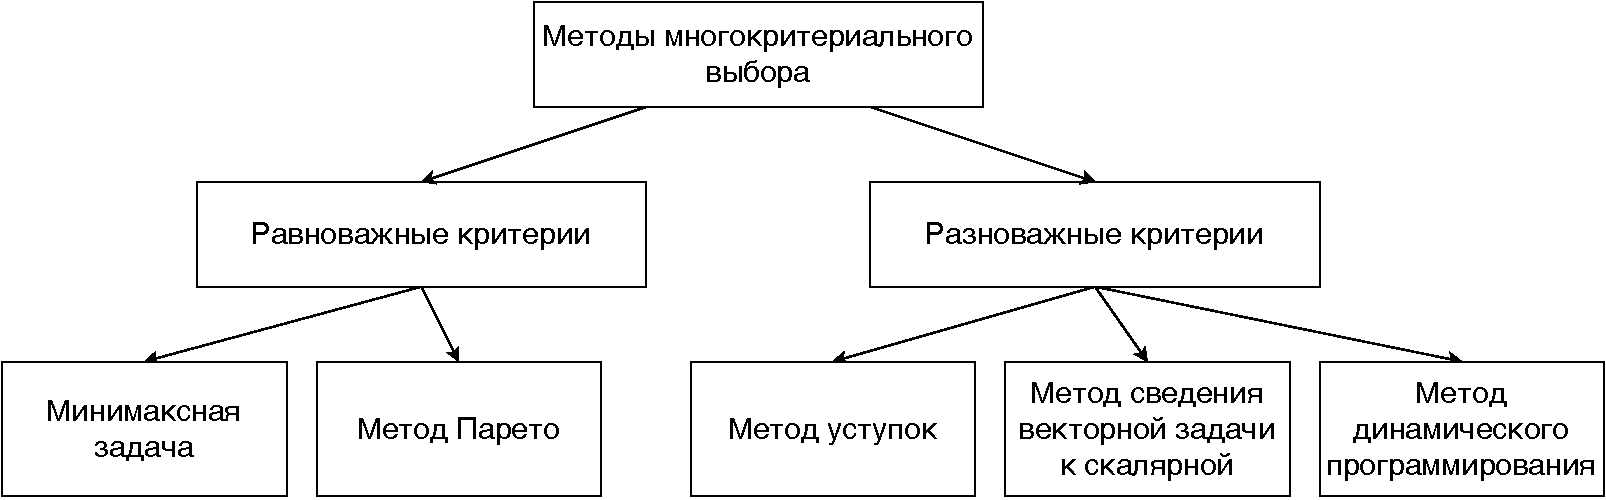
\includegraphics[scale=0.6]{img/class.pdf}
    \caption{Классификация методов многокритериального выбора}
    \label{img:class}
\end{figure}

\section{Вывод}

В данной части был определен критерий классификации методов многокритериального выбора и проведена их классификация.

\chapter{Области применения методов многокритериального выбора}
В данной части будут предложены наиболее подходящие области применения методов многокритериального выбора.

Изученные методы многокритериального выбора имеют обширную область применения ввиду своей общности. Для правильного выбора метода достаточно правильно формализовать задачу, для решения которой этот метод будет применяться. От правильной постановки задачи, определения критериев оценки и формализации ожидаемых реальзутов в большинстве своем и зависит выбор того или иного алгоритма.
Рассматривая каждый алгоритм в отельности, можно примерно формализовать задачу, для которой он должен применяться. 

Метод Парето в качестве результата дает множество альтернатив. Целесеобразно пользоваться разными множествами конкретных критериев и составить несколько множеств Парето, что позволит наблюдать разные варианты альтернатив, пока не выявится нужное множество альтернатив. Возможными областями применения для данного алгоритма могут служить:
\begin{itemize}[label=--]
    \item оценка надежности различного оборудования на предприятии \cite{bib9};
    \item выбор оптимальной дисконтной цены на товар \cite{bib12};
    \item выбор требований пожарной безопасности \cite{bib11};
    \item и т.д..
\end{itemize}

Минимаксная задача допустима в том случае, когда не требуется поиск оптимального множества альтернатив, а нужно найти одну определенную альтернативу. Данный метод применим в сферах определения характеристик производимых товаров, поиска чего-го либо и т.д.. \cite{bib13} \cite{bib14}

Метод уступок применим в тех случаях, когда требуется найти одно среднее решение, которое будет удовлетворять всем требованиям в целов. Сферы применения данного метода также обширны: решение задач расписания, выбора иструментов для рекламы и т.д..\cite{bib13} \cite{bib16}

Метод динамического программирования и метод сведения задач векторной оптимизации к задачам скалярной оптимизации ввиду своей декомпозиции до однокритериальной задачи применимы для задач, которые приследуют только одну цель. К таким задачам можно отнести: выбор стратегии управления или любая другая задача, которая приводит к однозначному исходу. \cite{bib10} \cite{bib17}

\section{Вывод}
В данной части были предложены наиболее подходящие области применения методов многокритериального выбора.

\chapter*{Заключение}
\addcontentsline{toc}{chapter}{Заключение}

В ходе данной работы были рассмотрены некоторые методы многокритериального выбора и была проведена их классификация.

Задачи, решенные  для достижения поставленной цели:
\begin{enumerate}[label=\arabic*)]
    \item рассмотрены математические основы теории принятия решений;
    \item проведен обзор многокритериальных задач и методов их решения;
    \item определен критерий классификации методов многокритериального выбора;
    \item классифицированы методы многокритериального выбора;
    \item предложены наиболее подходящие области применения.
\end{enumerate}

